\documentclass[psamsfonts]{amsart}

% -------Packages---------
\usepackage{microtype}[final]
\usepackage[style=numeric]{biblatex}
\usepackage{hyperref}
\addbibresource{/home/philip/documents/text/references/bibliography.bib}
\usepackage{amssymb,amsfonts}
\usepackage[all,arc]{xy}
\usepackage{enumerate}
\usepackage{mathrsfs}
\usepackage{todonotes}
\usepackage{tikz}
\usetikzlibrary{automata,positioning}
\usepackage[nolist]{acronym}

%--------Theorem Environments--------
%theoremstyle{plain} --- default
\newtheorem{thm}{Theorem}[section]
\newtheorem{cor}[thm]{Corollary}
\newtheorem{prop}[thm]{Proposition}
\newtheorem{lem}[thm]{Lemma}
\newtheorem{conj}[thm]{Conjecture}
\newtheorem{quest}[thm]{Question}
\newtheorem{prob}[thm]{Problem}

\theoremstyle{definition}
\newtheorem{defn}[thm]{Definition}
\newtheorem{defns}[thm]{Definitions}
\newtheorem{con}[thm]{Construction}
\newtheorem{exmp}[thm]{Example}
\newtheorem{exmps}[thm]{Examples}
\newtheorem{notn}[thm]{Notation}
\newtheorem{notns}[thm]{Notations}
\newtheorem{addm}[thm]{Addendum}
\newtheorem{exer}[thm]{Exercise}

\theoremstyle{remark}
\newtheorem{rem}[thm]{Remark}
\newtheorem{rems}[thm]{Remarks}
\newtheorem{warn}[thm]{Warning}
\newtheorem{sch}[thm]{Scholium}


\makeatletter
\let\c@equation\c@thm
\makeatother
\numberwithin{equation}{section}

\title{Undecidability and the structure of the Turing degrees}

\author{Philip Adams}

\date{\today}

\begin{document}

\begin{abstract}

  This paper explores the structure and properties of the Turing degrees, or
  degrees of undecidability. We introduce the Turing machine, an abstract model
  of computation, in order to develop the concepts of undecidability and Turing
  reduction. We demonstrate the technique of proof by reduction through a series
  of examples of undecidable problems related to context-free grammars. We then
  employ reducibility to consider a partial ordering on the set of Turing degrees, $\mathcal{D}$. Finally, we prove a variety of theorems
  related to the structure of $\mathcal{D}$.
  
\end{abstract}

\maketitle


\tableofcontents
\begin{acronym}
  \acro{PDA}[PDA]{Pushdown Automaton}
  \acroplural{PDA}[PDAs]{Pushdown Automata}
  \acro{DPDA}[DPDA]{Deterministic Pushdown Automaton}
  \acroplural{DPDA}[DPDAs]{Deterministic Pushdown Automata}
  \acro{TM}[TM]{Turing Machine}
  \acro{FSA}[FSA]{Finite State Automaton}
  \acroplural{FSA}[FSAs]{Finite State Automata}
  \acro{CFG}[CFG]{Context-Free Grammar}
  \acro{CFL}[CFL]{Context-Free Language}
\end{acronym}

\section{Introduction}
Historical overview of the field, motivation for study
\cite{ambos-spies06:_degrees_unsol}
\cite{soare16_turin_comput}
\cite{soare1999history}
\cite{lerman16:_degrees_unsol}
\subsection{Decision Problems}


\section{Turing Machines}
Upon consideration of different types of problems, it quickly becomes clear that
some are much more difficult than others. For example, when considering words
over the alphabet $\{a,b,c\}$, it seems much easier to determine whether a word
ends in an $a$ than whether a word is a palindrome. It seems even harder still
to determine whether the word is of the form $a^nb^nc^n$. In order to formalize
these notions of difficulty, we need to build abstract models of computation,
and then test their ability to decide such questions. We observe that a machine
that can solve the first problem only needs to ``remember'' the same amount of
information no matter how long the input is: the last letter of the word. In
contrast, the amount of memory that the second and third problems require is
dependent on the size of the input, because the first half of the palindrome or
$n$, respectively, can be arbitrarily large. The difference between the second
and third problems is more subtle: the second problem can be solved moving only
one direction in memory, while the third problem requires the ability to ``look
back'' in memory.
\par
Based on these differences, we can begin to construct different models of
computation that have just enough power to solve each problem. The first problem
can be solved by a \emph{\ac{FSA}}, a collection of a finite
number of states, a transition function, and a set of accepting states. The
\ac{FSA} accepts the input if the sequential application of each element to the
input finishes in an accepting state, and rejects otherwise. \aclp{FSA} are often represented by charts as in Figure~\ref{fig:fsa}, a
representation of an \ac{FSA} that decides the first problem.
\begin{figure}[h]
  \caption{An \ac{FSA} that determines whether a string ends in
    `$a$'.}
  \label{fig:fsa}
  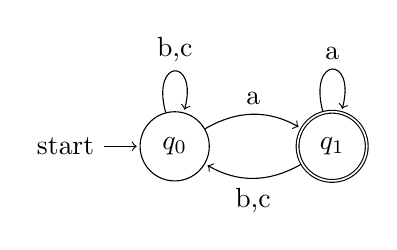
\begin{tikzpicture}[shorten >=1pt,node distance=2cm,on grid,auto]
  \node[state,initial] (q_0) {$q_0$};
  \node[state,accepting] (q_1) [right=of q_0]{$q_1$};
  \path[->]
  (q_0) edge [loop above] node {b,c} ()
  edge [bend left] node  {a} (q_1)
  (q_1) edge [bend left] node {b,c} (q_0)
  edge [loop above] node {a} ();
\end{tikzpicture}
\end{figure}
\par
The second problem can be solved by a machine called a \emph{\ac{PDA}}, which is essentially a finite state automaton with the addition of
a stack. Rather than transforming the current state and the input into a new
state, as with a finite state automata, the transition function of a \ac{PDA} also considers the stack, which it can pop and push from. Within the
collection of \acp{PDA}, there is another division between
\emph{\acp{DPDA}} and \emph{Nondeterministic \aclp{PDA}}. For \acp{DPDA}, the
transition function only outputs one move, rather than a set of
moves. Nondeterministic \acp{PDA} are able to recognize more languages than
\acp{DPDA}. Figure~\ref{fig:pda} is a graphical representation of a \ac{PDA}
that decides palindromes. In this representation, $\epsilon$ is an empty input,
and  is a special symbol that denotes the bottom of the stack. The moves are
represented by a double of input and stack operation.

\begin{figure}[h]
  \label{fig:pda}
  \caption{A \acl{PDA} that decides palindromes over the alphabet ${a,b}$}
  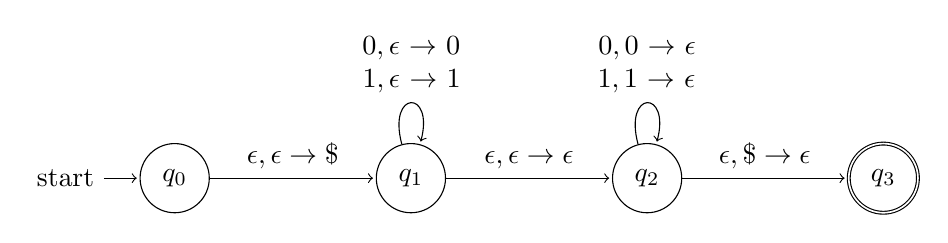
\begin{tikzpicture}[shorten >=1pt,node distance=3cm,on grid,auto]
  \node[state,initial] (q_0) {$q_0$};
  \node[state] (q_1) [right=of q_0]{$q_1$};
  \node[state] (q_2) [right=of q_1]{$q_2$};
  \node[state,accepting] (q_3) [right=of q_2]{$q_3$};
  \path[->]
  (q_0) edge node {$\epsilon,\epsilon\to\$$} (q_1)
  (q_1) edge [loop above] node[text width=1.5cm,align=center] {$0,\epsilon\to 0$
    $1,\epsilon\to 1$} ()
  edge node {$\epsilon,\epsilon\to\epsilon$} (q_2)
  (q_2) edge [loop above] node[text width=1.5cm,align=center] {$0,0\to\epsilon$
    $1,1\to\epsilon$} ()
  edge node {$\epsilon,\$\to\epsilon$} (q_3);  
  \end{tikzpicture}
\end{figure}
\par
Finally, we arrive at the \ac{TM}, devised by Alan Turing in his paper \emph{On
  Computable Numbers, With an Application To the Entscheidungsproblem}
~\cite{turing37_comput_number_with_applic_to_entsc}. \aclp{TM} offer an
unrestricted model of computation,\todo{Discussion of TMs}
\section{Undecidability}


\begin{prob}[The Halting Problem]
  \label{prob:halting}
  \cite{turing37_comput_number_with_applic_to_entsc}
  \cite{sipser13:_introd_theor_comput}
\end{prob}
\begin{thm}[Rice's Theorem] \cite{kozen99_autom}
  % Proof by reduction to the halting problem?
\end{thm}
\subsection{Incompleteness}
\begin{thm}[G\"odel's Incompleteness Theorem] 
  % Kleene 1943? Also shown in hopcroft 1979
  \cite{kleene43_recur_predic_quant}
\end{thm}
\subsection{Reducibility}
While it is possible to prove that a problem is undecidable directly, as in
problem~\ref{prob:halting}, it is often more convenient to prove undecidability
through comparison to problems which are already known to be undecidable. This
comparison takes place through the technique of Turing reduction.
\begin{defn}
  Given two decision problems $A$ and $B$, we say that $A$ is Turing reducible
  to $B$ if, given a machine $D_B$ that decides $B$, it is possible to construct
  a machine $D_A$ that decides $A$.
\end{defn}
So, we have that if $A$ is reducible to $B$, then $A$ can be no harder than $B$,
because any solution to $B$ also leads to a solution of $B$. So, if we have some
problem $B$ that we would like to prove is undecidable, we can do so by showing
that some problem $A$ which is already known to be undecidable is reducible to
$B$. Since $A$ cannot be harder than $B$, it follows that $B$ must also be
undecidable. Alternatively, if we would like to show that some problem $A$ is
decidable, it is sufficient to show that it is reducible to some problem $B$
that is known to be decidable.
\cite{sipser13:_introd_theor_comput}
\cite{post44:_recur}

\cite{kleene80_introd}

\section{Context Free Grammars}

\begin{defn}
 A Context Free Grammar is...
\end{defn}

\begin{defn}
  A Pushdown Automata is...
\end{defn}

\begin{thm}[Equivalence of CFGs and Pushdown Automata]
  \cite{hopcroft07:_introd_autom_theor_languag_comput}
\end{thm}
\begin{thm}[Closure Properties]
  \cite{sipser13:_introd_theor_comput}
  Union, Concat, Star, intersection with regular, substitution
\end{thm}
\begin{prob}[Emptiness]
  \label{prob:cfg:emptiness}
Let $G$ be a context-free grammar. Is $L(G)=\varnothing$?
\end{prob}

\begin{prob}[Finite]
Let $G$ be a context-free grammar. Is $L(G)$ finite?
\end{prob}

\begin{prob}[Regular Containment]
Take some context-free grammar $G$ and some regular language $R$. Is
$L(G)\subseteq R$?
\begin{proof}[Proof of Decidability]
  We have that $L(G)\subseteq R$ if and only if
  $\overline{L(G)}\cup R = \Sigma^*$. So, it follows that $L(G)$ is contained by
  $R$ if and only iff $\overline{\overline{L(G)}\cup R} = \varnothing$. By
  DeMorgan's laws, we have that this is equivalent to the statement
  $L(G)\cap \overline{R} = \varnothing$. Regular languages are closed under
  complement and context-free languages are closed under intersection with a
  regular language, so it follows that $L(G)\cap \overline{R}$ is a context free
  language. So the problem of containment by a regular language is reducible to
  Problem~\ref{prob:cfg:emptiness}, the problem of emptiness, which is
  decidable. So, the problem of containment by a regular language is decidable.
\end{proof}

\end{prob}

\subsection{Undecidable Problems}
\begin{prob}[The Post Correspondence Problem]
  Consider some alphabet $\Sigma$ and two finite lists of words over $\Sigma$
  denoted $A = a_1,\dots,a_n$ and $B = b_1, \dots, b_n$. Then, does there exist
some sequence of indices $(i_k),$ for $1 \leq k \leq K$ and for
  $K\geq 1$, and with $1 \leq i_k \leq n$ for all $k$ such that
  \[
    a_{i_1}\dots a_{i_K} = b_{i_1}\dots b_{i_K}?
  \]
  \begin{proof}[Solution]
    This problem is shown to be undecidable through a reduction to the halting
    problem. The proof is technical, and involves encoding the computation
    history of a Turing machine on an input in such a way that the encoding satisfies the
    PCP if and only if the Turing machine accepts the input. It is described in
    detail by Sipser in his book \emph{Introduction to the Theory of Computation}
    \cite{sipser13:_introd_theor_comput}.
  \end{proof}
\end{prob}

The Post correspondence problem is a useful tool, because it allows us to
demonstrate the undecidability of problems without doing the complex reasoning
about Turing machines that the halting problem requires. We will now show the
undecidability of a variety of problems about context-free grammars through
reduction to the Post correspondence problem.

\begin{prob}[Disjointness]
  Let $P,Q$ be context-free grammars. Is $L(P)\cap L(Q) = \varnothing$?
  \begin{proof}[Proof of Undecidability]
    Consider the Post correspondence problem for two lists of words $A,B$. We
    construct two context free grammars from these lists as follows:
    \begin{equation*}
      \begin{split}
        G_A \rightarrow  &\;a_11 \\
        &\!\!\!\!\vdots \\
        G_A \rightarrow  &\;a_nn \\
        G_A \rightarrow  &\;a_1G_A1 \\
        &\!\!\!\!\vdots \\
        G_A \rightarrow  &\;a_nG_An \\
      \end{split}
      \qquad
      \begin{split}
        G_B \rightarrow  &\;a_11 \\
        &\!\!\!\!\vdots \\
        G_B \rightarrow  &\;a_nn \\
        G_B \rightarrow  &\;a_1G_B1 \\
        &\!\!\!\!\vdots \\
        G_B \rightarrow  &\;a_nG_Bn \\
      \end{split}
    \end{equation*}
    Then, we can observe that for some string $s$ to exist in both $L(G_A)$ and $L(G_B)$,
    it must be a solution to the Post correspondence for $A,B$. So, if $L(G_A)\cap
    L(G_B)=\varnothing$, then there are no solutions to the Post correspondence
    for $A,B$. So, it follows that the Post correspondence problem is reducible
    to the problem of the disjointness of context-free grammars, so since the
    Post correspondence problem is undecidable, it follows that the disjointness
    problem is undecidable.
  \end{proof}
\end{prob}

\begin{prob}[Universality]
  \label{prob:cfg:universality}
  Let $G$ be some context-free grammar over an alphabet $\Sigma$. Then, is
  \[
    L(G) = \Sigma^*?
  \]
  \begin{proof}[Proof of Undecidability]
    
  \end{proof}
\end{prob}

\begin{defn}
An ambiguous grammar is...
\end{defn}

\begin{prob}[Ambiguity]
  Let $G$ be a context-free grammar. Is $G$ ambiguous?
  \begin{proof}[Proof of Undecidability]
    Consider the Post correspondence problem for two lists of words
    $A,B$. Construct their corresponding grammars $G_A,G_B$. Now, consider the
    grammar
    \[
      G \rightarrow G_A \vert G_B.
    \]
    It follows that the ambiguity of $G$ implies that a solution to the Post
    correspondence problem for $A,B$ exists, so the Post correspondence problem
    reduces to the ambiguity problem, so the ambiguity problem is undecidable.
  \end{proof}
\end{prob}
\cite{greibach66:_unsol_recog_linear_contex_free_languag}
\cite{Hopcroft1969}
\begin{prob}
  Let $G$ be a context free grammars. Is $L(G)$ regular?
  \begin{proof}[Proof of Undecidability]
    Note that $\Sigma^*$ is regular, so if $L(G)$ is not regular then it follows
    that $L(G)\neq \Sigma^*$. Additionally, universality is decidable within
    regular languages, because they are closed under complement and emptiness is
    decidable even within context-free grammars. So, we have that
    Problem~\ref{prob:cfg:universality} reduces to the regularity problem. It
    follows that the regularity problem is undecidable.
  \end{proof}
\end{prob}
\begin{prob}[Equality]
  Let $G_1,G_2$ be context free grammars. Is $L(G_1)=L(G_2)$?
  \begin{proof}[Proof of Undecidability]
    Note that $\Sigma^*$ is regular, so it is also a context-free. So,
    we have that Problem~\ref{prob:cfg:universality} reduces to the equality
    problem. It follows that the equality problem is undecidable.
  \end{proof}
\end{prob}
\begin{prob}[Inclusion]
  Let $G_1,G_2$ be context free grammars. Is $L(G_1)\subseteq L(G_2)$?
  \begin{proof}[Proof of Undecidability]
    As before, note that $\Sigma^*$ is regular, so it is also a
    context-free. Additionally, observe that for any grammar $G$, $L(G)\subseteq
    \Sigma^*$. So,
    we have that Problem~\ref{prob:cfg:universality} reduces to the inclusion
    problem, since $\Sigma^* \subseteq L(G) \implies \Sigma^* = L(G)$. It follows that the inclusion problem is undecidable.
  \end{proof}
\end{prob}

\subsubsection{Problems decidable for Deterministic CFLs}
\cite{ginsburg65:_deter}
\begin{defn}
  A deterministic context-free language is a language accepted by a
  deterministic pushdown automata.
\end{defn}

\begin{thm}[Closure Properties]
  If $L$ is a deterministic context-free language, then $\overline{L}$ is a
  deterministic context-free language.
\end{thm}

\begin{prob}
  Let $L$ be a deterministic context-free language. Is $L = \Sigma^*$?
\end{prob}

The decidability of the following problem was an open problem in the field of
computability theory from 1965, when it was introduced by Ginsburg and Greibach \cite{ginsburg65:_deter}. In 1997, when it was solved by G\'eraud S\'enizergues
\cite{senizergues_det_pd_decid}. A sketch of the proof follows. 

\begin{prob}[The Equivalence Problem for Deterministic CFGs]
  Let $L_1,L_2$ be deterministic context-free languages. Is $L_1=L_2$?

\end{prob}

\section{Turing Degrees}
\begin{defn}
  A Turing degree...
\cite{post44:_recur}
\cite{kleene54_upper_semi_lattic_degrees_recur_unsol}
\end{defn}

\begin{defn}
  The jump operator...
  
\end{defn}

\begin{defn}
  Computably Enumerable
\end{defn}

\begin{defn}
  Completeness
\end{defn}

\subsection{Properties and Structure}
\begin{prob}[Post's Problem]
  \cite{post44:_recur}
  % Marchenkov 1976
  % Independently by Friedberg 57, Mucnik 56/58 using priority method
  % Priority free solution Kucer 1986''
  % ``Natural'' solns don't exist
  \cite{Friedberg236}
\end{prob}

% Myhill 56 c.e.lattice

\begin{lem}
  D does not form a lattice
  \cite{kleene54_upper_semi_lattic_degrees_recur_unsol}
\end{lem}
\begin{thm}
  D forms an upper semi-lattice
  % Kleene-Post 54 Degrees upper semi-lattice, jump an operator on degrees
  \cite{kleene54_upper_semi_lattic_degrees_recur_unsol}
\end{thm}

\begin{thm}
  Existence of minimal degrees
  % Spector 56,Shoenfield 66 (Better)
  \cite{spector56_degrees_recur_unsol}
  \cite{shoenfield66_theor_minim_degrees}
\end{thm}

\begin{thm}
  The c.e. degrees are dense
  \cite{sacks64:_recur_enumer_degrees_dense}
\end{thm}

Homogeneity problems
% Feiner 1970, Shore 1979

Theory of D Undecidable

\subsection{Turing Degrees of Problems related to CFGs}
\cite{REEDY197577}




\section*{Acknowledgments}
It is a pleasure to thank my mentor, Ronno Das, for supervising this project and
providing valuable feedback and advice. I would also like to thank Peter May for
organizing this REU, and Daniil Rudenko for running the Apprentice Program.

\printbibliography

\end{document}


%%% Local Variables:
%%% mode: latex
%%% TeX-master: t
%%% End:
